\documentclass[a4paper,oneside,12pt,titlepage]{article}

% Packages
%\usepackage[utf8]{inputenc}	% Zeichenkodierung
\usepackage[ngerman]{babel}
\usepackage{a4wide}		% Papierformat
\usepackage{lmodern}		% Schriftarten
\usepackage{graphicx}	% Formatierung
\usepackage{amsmath}		% Mathe Fonts
\usepackage{amsfonts}	% Fonts
\usepackage{tikz}		% Zeichnen von Grafiken
\usepackage{listings}	% Code listings
\usepackage{courier}		% Code Font
\usepackage{xcolor}		% Advanced Color
\usepackage[backend=bibtex]{biblatex}
\usepackage[babel]{csquotes}
\usepackage[top=1.5in, bottom=1in, left=1.25in, right=1.25in]{geometry}
\usepackage{float}
\usepackage{fontspec}

% Farbdefinition
\definecolor{link}{HTML}{3333FF}			% Link
\definecolor{mygreen}{rgb}{0,0.6,0} 		% Listings
\definecolor{mygray}{rgb}{0.5,0.5,0.5}	% Listings
\definecolor{mymauve}{rgb}{0.58,0,0.82}	% Listings
\colorlet{punct}{red!60!black}			% Listings
\definecolor{background}{HTML}{EEEEEE}	% Listings
\definecolor{delim}{RGB}{20,105,176}		% Listings
\colorlet{numb}{magenta!60!black}		% Listings
% Ende Farbdefinition

% Einstellungen
\renewcommand*{\familydefault}{\sfdefault}	% Default Font
\setmonofont[Ligatures=Common, Scale = 0.8, Path = fonts/]{firecode.otf}
\renewcommand{\abstractname}{}				% Überschrift Abs.
\linespread{1.1}					% Zeilenabstand
\usepackage{listings}
\usepackage{xcolor}

\colorlet{punct}{red!60!black}
\definecolor{background}{HTML}{EEEEEE}
\definecolor{delim}{RGB}{20,105,176}
\colorlet{numb}{magenta!60!black}

\lstdefinelanguage{json}{
    basicstyle=\normalfont\ttfamily,
    numbers=left,
    numberstyle=\scriptsize,
    stepnumber=1,
    numbersep=8pt,
    showstringspaces=false,
    breaklines=true,
    frame=lines,
    backgroundcolor=\color{background},
    literate=
     *{0}{{{\color{numb}0}}}{1}
      {1}{{{\color{numb}1}}}{1}
      {2}{{{\color{numb}2}}}{1}
      {3}{{{\color{numb}3}}}{1}
      {4}{{{\color{numb}4}}}{1}
      {5}{{{\color{numb}5}}}{1}
      {6}{{{\color{numb}6}}}{1}
      {7}{{{\color{numb}7}}}{1}
      {8}{{{\color{numb}8}}}{1}
      {9}{{{\color{numb}9}}}{1}
      {:}{{{\color{punct}{:}}}}{1}
      {,}{{{\color{punct}{,}}}}{1}
      {\{}{{{\color{delim}{\{}}}}{1}
      {\}}{{{\color{delim}{\}}}}}{1}
      {[}{{{\color{delim}{[}}}}{1}
      {]}{{{\color{delim}{]}}}}{1},
}				% Define JSON Language
\lstset{							% Listing Settings
breaklines=true,					% Wrap
commentstyle=\color{mygreen},	% Comment Color
showstringspaces=false,			% Show _ Space
extendedchars=true,				% Umlaute
keywordstyle=\color{blue},		% Keywords
tabsize=3,						% Tabs in Spaces
stringstyle=\color{orange},		% String color
basicstyle=\normalfont\ttfamily,	% Font
numbers=left,					% Numberside
numberstyle=\scriptsize,			% Numbersize
stepnumber=1,					% Linenumbering
numbersep=8pt,					% Margin Right
frame=lines,						% Line top/bottom
backgroundcolor=\color{background},	% Background Color
}
\usetikzlibrary{shapes,arrows}	% For Flow Diagram
\bibliography{quellen}
% Ende Einstellungen

% Sprachdefinition
\lstdefinelanguage{grads}{
 keywords=[0]{
   while, endwhile, if, endif, function, return,
 },
 keywords=[1]{
   substr, subwrd
 },
 morestring=[b][\color{orange}]{"},
 morestring=[b][\color{red}]{'},
 morecomment=[l]*,
 sensitive=true,
 breaklines=true,
 extendedchars=true
}
% Ende Sprachdefinition

% Shortcuts
\newcommand{\jf}{Jugend forscht }
\newcommand{\vs}{ViSys}
\newcommand{\mb}{Markus Becker}
\newcommand{\sw}{TOBEREMOVED}
\newcommand{\re}{Dr. Ronald Eixmann}
\newcommand{\tw}{Thoralf Wieck}
\newcommand{\thema}{Personalisierte Datenverarbeitung\\und Visualisierung von Wetterprognosedaten}
\newcommand{\pyvidir}{../../Code/PyVi/}	% Relativ zu auvi/Latex/Lernleistung
\newcommand{\demodisdir}{../../Code/Anzeige/ort/}
% Ende Shortcuts

% Variablen
% ...
% Ende Variablen

% Eigene Befehle
\newcommand{\link}[1]{\textcolor{link}{#1}}	% Format Links
\newcommand{\jftree}{\begin{center}
\scalebox{0.56}{
\begin{tikzpicture}[
every node/.style = {scale=1.2},
level 1/.style = {sibling distance = 8.5cm},
level 2/.style = {sibling distance = 3cm},
level 3/.style = {sibling distance = .5cm},
level distance = 1.25cm
]
\node {\LARGE \textbf{AuVi}}
    child { node {\large \vs}
        child { node {Programmierung}}
        child { node {Servertechnik}
            child { node {Schnittstelle}}
        }
        child { node {Meteorologie}
            child { node {Datenquellen}}
        }
    }
    child { node {\large Makanya.com}
        child { node {Konzept}}
        child { node {Sicherheit}}
        child { node {Sprache}}
    }
    child { node {\large Weather Monitoring System}
        child {node {Interface}}
        child {node {Sicherheit}}
        child {node {Erreichbarkeit}}
    };
\end{tikzpicture}
}
\end{center}}	% Draw JF Tree
% Ende Eigene Befehle

\begin{document}

% Titelseite
\pagestyle{empty}
\title{
\includegraphics[scale=.34]{imgs/auvi_white.png}\\\thema}
\author{Schüler:\\\mb \and Projektbetreuer:\\\re\\\tw}
\maketitle
% Ende Titelseite

\newpage
\Large{Selbstständigkeitserklärung}\\
\\
\small Hiermit erklären wir,
dass wir die vorliegende Arbeit selbständig angefertigt,
nicht anderweitig zu Prüfungszwecken vorgelegt und keine anderen,
als die angegebenen Hilfsmittel verwendet haben.
Zudem waren alle verwiesenen Webseiten zum Zeitpunkt der Linksetzung gültig und erreichbar.
Wörtlich und sinngemäße Übernahmen aus anderen Werken sind als solche gekennzeichnet.
\\
\newpage

% Inhaltsangabe
\pagestyle{empty}
\tableofcontents
\thispagestyle{empty}
\pagestyle{plain}
\newpage
% Ende Inhaltsangabe


\pagestyle{headings}
\markright{\thesection\hfill\thepage}
\renewcommand{\sectionmark}[1]{ \markright{#1}{} }
\newcommand{\headrulewidth}{0.5pt}
\newcommand{\footrulewidth}{0pt}

\begin{abstract}
\jftree
Mit \textbf{AuVi} bezeichnen wir eine Gruppe von verschiedenen Projekten unter der Leitung von Ronald Eixmann.
Die Projektarbeit findet von Markus Becker und Swenja Wagner statt.
Unser zentrales Projekt gibt unserer Arbeit ihren Namen. AuVi steht für Automatisierte Visualisierung von meteorologischen Daten, dem Projekt mit dem wir an verschiedensten \jf Wettbewerben teilnahmen.
Dieses ermöglicht einem Nutzer über eine Website oder App eine Wetterprognose für jeden beliebigen Punkt auf der Erde mit über 50 verschiedenen Parametern abzufragen.
Diese Prognose kann bis zu zehn Tage in die Zukunft abgegeben werden.\\
Später wurde unsere Projektarbeit um eine Partnerschaft mit Makanya erweitert.
So entstand Makanya.com, eine Website um einen Austausch zwischen Schülern aus Deutschland und Tansania zu ermöglichen.\\
Der letzte teil unseres Projektes ist das Weather Monitoring System rund um Kühlungsborn.
Dieses umfasst eine Reihe von Bildschirmen die Wetterdaten sowie aktuelle Informationen anzeigen.
Gleichzeitig wird das System allerdings auch von der Schule genutzt um Informationen im Foyer anzuzeigen.\\
All diese Teilprojekte sind natürlich auch mit Öffentlichkeitsarbeit verbunden.
\end{abstract}


\section{Auvi}

\subsection{Programm} % AuVi
Um Verwechslungen zu verhindern benenne ich das Programm,
welches ich unter AuVi entwickelt habe ,,\vs ''.
Der Kürzel steht für Visualisierung System und ist in verschiedenen Versionen lauffähig.
Die Aufgabe von \vs\ ist es auf eine Datenquelle zuzugreifen
und nach abgespeicherten Parametern die Rohdaten in Grafiken umzuwandeln.
Dabei wird von mir sehr viel Wert darauf gelegt,
dass das Erstellen der Grafiken möglichst abstrakt behandelt wird,
damit der Nutzer sehr großen Einfluss auf das Design und den Inhalt der Grafiken nehmen kann.

\subsection{Meteorologie} % AuVi

\subsubsection{Prognosetheorie} % AuVi Meteorologie
Die Meteorologie gehört zu den Naturwissenschaften und
beschäftigt sich mit der Atmosphäre, der Wetterprognose und der Klimatologie \cite{meteorologie}.
Sie liefert somit die Voraussetzungen um eine Wettervorhersage erstellen zu können.
Unter einer Wetterprognose versteht man die Vorhersage eines Zustands
der Atmosphäre zu einem bestimmten Zeitpunkt an einem bestimmten Ort
oder in einem bestimmten Gebiet.
Es wird nicht nur das Wetter in Bodennähe betrachtet,
sondern auch Wettererscheinungen in höheren Schichten der Erdatmosphäre.
\\
Das Wetter lässt sich durch entsprechende Naturgesetze beschreiben.
Das ist für die Prognose essentiell wichtig.
Der Grundgedanke einer solchen Prognose besteht darin,
aus einem bereits vergangenen und dem aktuellen Zustand
der Atmosphäre einen Zustand in der Zukunft abzuleiten.
Dazu werden die bekannten physikalischen Regeln angewendet.
In mathematischer Hinsicht werden diese physikalischen Regeln von
nichtlinearen Gleichungen beschrieben.
Das bedeutet, dass bereits die kleinste Änderung im Ausgangszustand
das Ergebnis der Rechnung relativ groß verändern kann. % TODO: Citation needed


\subsubsection{Prognosen per Hand} % AuVi Meteorologie
Was muss man über die aktuelle Situation wissen um per Hand eine Prognose zu erzeugen?
Es gibt einen Unterschied zwischen der manuellen oder auch
synoptischen Wettervorhersage und einer numerischen Wettervorhersage.
In der synoptischen Meteorologie ist ein System aus Beobachtungsstationen
nötig, die gleichzeitig Wetterbeobachtungen nach einem einheitlichen Verfahren durchführen.
Die Stationen messen unter anderem Parameter wie:
Luftdruck, Luftdruckänderung während der letzten drei Stunden,
Lufttemperatur, Windrichtung, Windgeschwindigkeit, Taupunkt,
Wolkenart, Höhe der Wolkenuntergrenze, Bedeckungsgrad,
Sichtweite, Niederschlagsmenge und Niederschlagsart.
Es wird zwischen Bodenbeobachtungsstationen, die Daten in der Nähe
der Bodenoberfläche sammeln und aerologischen Beobachtungsstationen,
die Daten aus bis zu 30km Höhe liefern unterschieden.
Es werden auch Daten von mobilen Messstationen, wie Bojen und Flugzeugen verwendet.
Wettersatelliten und Fernerkundungssystem
(wie Wetterradar, Blitzortungssysteme, LIDAR, SODAR) können auch als Datenquelle dienen.
Die gesammelten Daten, die den Wetterzustand zu einem bestimmten
Zeitpunkt beschreiben, werden in Wetterkarten eingetragen.
Mit Hilfe der eingetragenen Daten werden die Wetterverhältnisse
analysiert und Wettervorhersagen erstellt.
Zusätzlich dazu werden die gesammelten Daten von numerischen
Vorhersagemodellen als Ausgangszustand verwendet. %[2]
\\
Numerische Wettervorhersagen sind rechnergestützt, müssen aber trotzdem nicht 100\% zutreffend sein.
Der Zustand der Atmosphäre zu einem späteren Zeitpunkt wird aus dem Zustand
der Atmosphäre zu einem gegebenen Anfangszeitpunkt berechnet.
Dabei werden relevante Gleichungen numerisch gelöst
(Navier-Stokes-Gleichung, thermische Zustandsgleichung idealer Gase,
erster Hauptsatz der Thermodynamik, Kontinuitätsgleichung).
Mit diesen Gleichungen werden Vorgänge, wie zum Beispiel Wolkenbildung,
Niederschläge, Bildung von Hoch- und Tiefdruckgebieten und Wind beschrieben.
Diese Vorgänge können je nach Luftdruck, Temperatur, Windgeschwindigkeit
und Luftfeuchtigkeit auftreten.
Da diese Gleichungen jedoch nicht eindeutig lösbar sind oder es
durch Approximationsvorgänge zu Abweichungen kommt, kann es nur zu Näherungswerten kommen.
Trotzdem, oder gerade deshalb sind diese numerischen Prognosen in unseren Rechenzentren berechenbar.
Diese mathematischen Näherungen benötigen jedoch sehr viel Rechenleistung,
weswegen auf die Leistungsfähigkeit von Supercomputern zurückgegriffen wird.
Bei solchen numerischen Vorhersagemodellen wird das betrachtete Gebiet in Gitterzellen unterteilt.
Für jeden Punkt werden dann die Parameter errechnet.
Relevante physikalische Größen sind vor allem Temperatur,
Luftdruck, Dichte, Windrichtung und Windgeschwindigkeit.
Es wird zwischen Global- und Lokal- oder Ausschnittsmodellen unterschieden.

\subsubsection{Voraussetzung für Wetterprognosen} % AuVi Meteorologie
Um Wetterprgnosen erstellen zu können, braucht man gewisse Ausgangswerte.
Die Ausgangsdaten bestehen aus Werten,
die an dem Punkt zu einem früheren Zeitpunkt gemessen wurden.
Die Entwicklung der verschiedenen Wettergrößen wird durch Formeln errechnet.
Diese Berechnung benötigt, wie oben schon erwähnt, eine enormer Rechenleistung.
Deswegen ist man für die Vorhersage von Wetterverhältnissen auf
die Hilfe eines leistungsfähigen Computers angewiesen.
Die entstandenen Modellergebnisse bilden die Basis, und können nun
von Prognostikern interpretiert und beurteilt werden.
Die Prognostiker können die Modelle anhand von aktuell gemessenen Werten
oder Bildern einer Webcam überprüfen und eine Vorhersage formulieren.
Dabei spielen das Wissen und die Erfahrungen der Prognostiker eine große Rolle.
Die Genauigkeit einer Wettervorhersage ist von der Stabilität der Wetterlage abhängig.
Bei wechselhaftem Wetter ist die Vorhersage deutlich schwieriger
und komplizierte als bei stabilen Wetterlagen.
Die Länge der Prognose spielt auch eine Rolle.
Es macht einen Unterschied,
ob man nur die Prognose für den nächsten Tag,
oder ob man die Prognose für die nächste Woche haben möchte.
Letzters ist deutlich schwieriger und somit auch weniger zuverlässig.

\subsection{Datenquellen} % AuVi

\subsubsection{Quellenvergleich} % AuVi Datenquellen
Da ich nun dargestellt habe, dass es für mich nicht möglich ist
eigene Daten aufzunehmen und Prognosen zu berechnen,
zeige ich nun welche Quellen die benötigten Daten zur Verfügung stellen.
Im Internet gibt es eine vielzahl von Anbietern von Wetterdaten.
Die seriöseste Methode an diese Daten zu gelangen ist über einen OpenDap Server.
Dieser garantiert dem Programmierer und somit dem Nutzer
die Erreichbarkeit und Aktualität der Daten.
Für mein Programm sammelte ich nun verschiedene Quellen und verglich sie untereinander.
Bei diesem, bei weitem nicht vollständigen Vergleich,
gewann die NOAA GFS Quelle \cite{noaa} , auf die ich durch Dr. Ronald Eixmann stieß.
Das GFS \cite{gfs} Modell welches von NOAA angeboten wird zeichnet
sich durch eine Vielfalt von Parametern (50+) und einen großen Prognosezeitraum (10 Tage) aus.
In \vs\ kann der Nutzer selbst zwischen den verschiedenen Datenquellen wählen und eigene hinzufügen.
Da die Software unter der MIT-Lizenz von mir im Internet veröffentlicht wurde,
und diese Lizenz die ,,As is - Klausel''
\footnote{Die Software wird von mir frei angeboten, darf verändert werden,
aber ich stehe nicht gerade für Fehler oder Abstürze} enthält verschreibe
ich mich keiner Garantieleistung \cite{mitl}. Ich kann somit Quellen
auflisten die in Zukunft evtl. nicht mehr erreichbar sind.
Ich strebe an über eine GUI\footnote{\textit{Graphical User Interface} engl. IT.
für grafische Benutzeroberfläche} dem Nutzer eine Auswahl
zwischen verschiedenen Datenquellen anzubieten.
% TODO: Grafik: Übersicht über Quellen (Alle die direkt über das Programm angeboten werden)
% NOTE Viel mehr Parameter, Daten bei NOAA oc DWD
% Siehe andere Quellen


\subsubsection*{Wetterdienst} % AuVi Datenquellen
% TODO Grafik: Diagramm der Genauigkeit (Dafür Tabelle, Swenja)
Der Deutsche Wetter Dienst, kurz: DWD, arbeitet im Auftrag des
Bundesministeriums für Verkehr und digitale Infrastruktur. \cite{bmvi}
Der DWD bietet ebenfalls Wetterdaten an, die allerdings kostenpflichtig sind.
Das Angebot ist unterteilt in ,,Aktuelles Wetter, Vorhersagen''
und ,,Vergangenes Wetter, Klimainfos''.
Im ersten Bereich gibt es zum Beispiel den Unterpunkt Seewetter.
Es wird ein Kurzfrist-Seewetterbericht,
Küstenwetter in Zeitreihenform und ein Mittelfrist-Seewetterbericht
für 48h für je 2,50 Euro angeboten.
Wenn man aus dieser Quelle alle zwei Tage eine Wetterprognose
bezieht - welche im Parameter stark eingeschränkt ist - belaufen
sich die Kosten auf ungefähr $\approx 230$ Euro.
Diese Wetterdaten können dann zum Beispiel für die Seefahrt genutzt werden.
Ein anderer Unterpunkt ist Flugwetter.
Dort gibt es Einjahresangebote für circa 80 Euro und Lehrfilmreihen für circa 150 Euro.
Diese dienen als Dokumentation.
Die Nutzer dieser Leistungen sind vermutlich größere Flughäfen.
Ein weiterer Bereich in dem Jahresabos und Monatsabos angeboten werden, ist Agrarwetter.
Die Kosten dafür belaufen sich auf 20 bis 120 Euro.
Der wohl interessanteste Unterpunkt ist Straßenwetter.
Da werden einmalige Informationen für allgemeine Wettervorhersagen für Straßen (4,40 Euro),
für detaillierte Gebietswettervorhersagen für Straßen
(4,40 Euro) und für Straßenwettervorhersagen für eine Stadt (5 Euro) dargeboten.\\
Im zweiten Bereich gibt es die genaueren Eingrenzungen
,,Deutschland - Allgemein'', ,,Deutschland - Speziell'' ,
,,Global'' und ,,Geburtstagswetterkarte''.
\cite{dwd-shop}
Diese Daten sind für uns allerdings nicht relevant, weil sie in der Vergangenheit liegen.\\
Da diese Quelle sich auf lange Zeit für uns als zu kostspielig herausgestellt hätte,
und auch die Datenmenge nicht für jeden Punkt der Erde definiert ist,
war für mich frühzeitig klar, dass ich eine alternative Quelle suchen musste.

\subsubsection*{NOAA Global Forecast System} % AuVi Datenquellen
Das Global Forecast System (GFS)  ist ein Modell, das mathematisch Parameter errechnet.
Es ist also ein numerisches Vorhersagemodell.
Die dazu benötigten Daten bezieht es aus einem Netz von Wetterstationen,
die sowohl an Land als auch im Wasser und in der Luft Messungen durchführen.
Mit diesen gemessenen Daten werden mithilfe von geophysikalischen Gesetzen weitere Daten errechnet.
So wird in einem Abstand von 13,5km je ein Wert ermittelt.
Diese Daten werden als große Datensätze kostenfrei auf
der Webseite \link{http://mag.ncep.noaa.gov/} \cite{ncep} zur Verfügung gestellt.\\
Im Verlauf meiner Arbeit vergliche ich verschiedene Quellen.
Auch wenn ich die Möglichkeit habe unter Angabe des Links mit einer
Einstellung eine andere Quelle zu benutzen habe ich mich
für das GFS Modell von NOAA als Haupt- und Standartquelle entschieden.
Das GFS ist zuverlässig und gut dokumentiert, was uns die Einarbeitung erleichterte.
Zudem bietet NOAA verschiedenste Varianten des GFS-Models an,
somit kann ich stark mitbestimmen welches Datenformat von der Software verwendet wird.
Die Daten liegen in verschiedenen zeitlichen und räumlichen Auflösungen vor.
% TODO Tabelle mit Daten: http://www.ftp.ncep.noaa.gov/data/nccf/com/gfs/prod/
% TODO Auflösungen heraussuchen http://www.nco.ncep.noaa.gov/pmb/products/gfs/
% Richtige Quelle
% http://opendap.nccs.nasa.gov:80/dods/GEOS-5/fp/0.25_deg/fcast/tavg1_2d_slv_Nx.latest
% TODO Quellenvergleich http://opendap.nccs.nasa.gov/dods/
% TODO Dokumentation Formate, GRIB2 (http)
% TODO Diagramm der Genauigkeit

\subsubsection{Datenverfügbarkeit} % AuVi Datenquellen
% TODO Wann sind welche Daten Verfügbar?
Während der Deutsche Wetter Dienst für normale, zahlende, Nutzer nur Daten
für die nächsten 48 Stunden zur Verfügung stellt, ist NOAA für alle Nutzer,
egal wo sie sich auf der Welt befinden, rund um die Uhr offen und bietet Daten
für die nächsten 10 Tage. Hierin unterscheiden sich allerdings die verschiedenen
Modelle des NOAA. Die statistischen oder historischen Daten sind immer Verfügbar.
Da sie die Vergangenheit beschreiben oder eine Reihe von Standaufnahmen darstellen
ist hier die Frage nach Datenverfügbarkeit weniger wichtig.\\
Unsere Arbeit behandelt haben hauptsächlich die Wetterprognose, bzw. die Auswertung
von Wetterprognosedaten. Für unsere Zwecke und Ziele ist Datenverfügbarkeit von
hoher Wichtigkeit. Ich muss erwarten können, dass die von mir verlangten Daten auch
dort verfügbar sind, wo sie sein sollen, und die Daten enthalten die nach der
Spezifikation enthalten sein sollen.\\
Diese Spezifikation der NOAA Daten steckt sich bei verschiedenen Modellen
verschiedene Ziele ab. Das von uns am meisten genutzte Modell, das GFS Modell ist
24-7 erreichbar, kostenlos und enthält Daten entweder für die nächsten 33 Stunden,
133 Stunden oder 240 Stunden.

\subsection{Entwicklung} % AuVi

\subsubsection{Wahl der Umgebung}\label{sec:ent} % AuVi Entwicklung
Bei der Entwicklung von AuVi wechselte mehrmals die Entwicklungsumgebung und die
genutzten Werkzeuge um Neugelerntes anzuwenden, oder die Arbeitsweise zu optimieren.
Außerdem wurden verschiedene Teile meiner Software in verschiedenen Programmiersprachen
geschrieben. Diese verlangten dann von mir ein Anpassen der Umgebung.\\
In heutiger Zeit unausweichlich ist der Wechsel der Hardware in einem Project,
welches über 3 Jahr läuft und sich zum Teil auf privaten Mitteln stützt. Dies
bedeutet in meinem Fall der Wechsel von Laptops, Computern und Betriebssystemen.\\
Der entscheidenste Wandel war die Migration aller Dateien in ein Git-Repository \cite{gitrepo}.
Dieser Wandel ermöglichte die potentielle Zusammenarbeit mit Projektteilnehmern, oder
dem Projektleiter ohne das von mir vorrausgesetzt wird, dass dieser die selben Möglichkeiten
auf seinem Rechner hat. Durch die Integration in GitHub kann der Quelltext auch auf
\link{github.com/tibyte/auvi-hub} aufgerufen werden. Mit einem Account auf dieser
Seite können dann u.a. Zeilen kommentiert werden. \\
Die Textbearbeitung fand zuerst im Editor Sublime Text \cite{sublime} statt, da dieser
aber kostenlos nur mit störenden Nachrichten zu nutzen war, wechselte ich später
zum Open Souce Atom Editor \cite{atomio}. Dieser wird von der GitHub Gemeinde entwickelt.
% TODO Beschreibung der Umgebung & Warum

\subsubsection{Methodik} % AuVi Entwicklung
Insofern keine anderen Informationen gegeben sind,
gilt diese Arbeitsweise in allen anderen Projektteilen. \\
Die Arbeit an diesem Projekt verlangte große Kooperation
von den verübergehenden Projektteilnehmern.
Treffen wurden geplant und üblicherweise auf den Dienstag Nachmittag gelegt.
Bei diesen Treffen wurde dann über neue Fortschritte geredet,
damit alle auf dem gleichen Wissensstand sind.
Ich habe mich dann mit den Anderen über Ideen ausgetauscht
und die nächsten Arbeitsschritte geplant.
Nach dem Austauschen haben ich dann am Projekt weitergearbeitet und Zuarbeit erhalten.
Doch reichten zwei bis drei Stunden in der Woche nicht aus um das Projekt zu bearbeiten.
Viele Arbeitsstunden mussten von zu hause erledigt werden.\\
Im Winter des Jahres 2013 absolvierten ich zusammen mit Swenja Wanger ein Schülerpraktikum am
Leibnitz Institut für Atmoshpärenphysik.
Dort nutzten ich die Möglichkeit um mit anderen dort arbeitenden
Wissenschaftlern über unser Projekt zu reden.
Hier entstand die erste lauffähige Version unseres Programmes.
Außerdem entwarf ich mehrere Poster für den \jf Wettbewerb 2014.

\subsubsection{Programmierung}
Die umfangreichste Aufgabe die ich in der Projektarbeit bewältigte
war die Programmierung der Software ,,\vs ''.
Da ich mich in Punkt \ref{sec:ent} schon entschieden habe in einer Linux Umgebung zu arbeiten,
mussten ich auch die Programmiersprachen und sowie IDE's so wählen,
dass sie auch auf Ubuntu oder ähnlichen Distributionen ohne Komplikationen funktionierten.\\
Unser Hauptprogramm, genannt ,,\vs '' haben ich erst in
Python (Version 2.7) \cite{python27} geschrieben.
Vorher gab es eine Ansammlung von Befehlen in einer BASH Datei welche die selbe Aufgabe
erfüllte. Diese Datei war sehr undynamisch und konnte auch schlecht auf verschiedene
Umgebungen reagieren.
Entschieden uns aber später unsere Fortschritte von Python Version 2.7 auf die Version 3 gehoben.
Diese Programmiersprache ist in den von uns genutzten Distributionen
sogar vorinstalliert und ein allgemeiner Industriestandard.\\
Nur mit Python kam ich allerdings auf lange Zeit nicht aus.
Ich nutzte noch andere Sprachen um die Entwicklung zu beschleunigen,
auch wenn Python für die restlichen Aufgaben auch hätten erfüllen können
kombinierte ich folgende Programmiersprachen:
\begin{figure}[H]
\begin{center}
\scalebox{0.7}{
\begin{tikzpicture}[
every node/.style = {},
level 1/.style = {sibling distance = 6cm},
level distance = 2cm
]
\node {\LARGE PyVi$=$\vs}
    child { node {\large Python} 
    		child { node{Flow, Management und IO}}
    }
    child { node {\large Bash}
    		child { node {Files, convert(ImageMagick)}}
    }
    child { node {\large PHP, HTML, JavaScript}
    		child { node {Website, Scripting}}
    }
    child { node {\large GrADS} 
    		child { node{Interpretieren der Rohdaten}}
    };
\end{tikzpicture}
}
\end{center}
\label{fig:pyvi}
\caption{Benutzte Programmiersprachen}
\end{figure}

\subsubsection*{Hauptprogramm}
\lstinputlisting[language=Python,firstline=12, lastline=41,firstnumber=12,caption={,,Mainfunktion'' von \vs\ (auvi.py)}]{\pyvidir auvi.py}
\lstinputlisting[language=Python,caption={Konstanten (local.py)},firstline=3,lastline=7,firstnumber=3]{\pyvidir local.py}
\lstinputlisting[language=Python,caption={Hinzufügen von neuen Orten, Gebieten und Parametern (local.py)},firstline=11,lastline=28,firstnumber=11]{\pyvidir local.py}
\lstinputlisting[language=Python,caption={Routine zum schreiben von JSON Dateien (local.py)},firstline=30,lastline=41,firstnumber=30]{\pyvidir local.py}
\lstinputlisting[language=Python,caption={Datei In- und Output (filemanager.py)},firstline=39,lastline=66,firstnumber=39]{\pyvidir filemanager.py}
\lstinputlisting[language=Python,caption={Umwandeln von Konturplots in Gif Dateien (filemanager.py)},firstline=68,lastline=80,firstnumber=68]{\pyvidir filemanager.py}

\subsubsection*{JSON Definitionen}
Im folgenden Listing wird die Definition von Ortspunkten
\footnote{Ortspunkte stehen im Kontrast zur Gebietsdefinition. Gebiete werden durch minimale Breiten- und Höhengrade definiert und besitzen eine Breite und Höhe. Anwendungsbeispiel: Europa, Welt, Asien, ...} gezeigt.
Diese werden im JSON Format gespeichert.
Die Liste kann um beliebig viele andere Orte erweitert werden.
\lstinputlisting[language=json, caption={Beispielobjekte für Ortspunkte (locals.json)}]{\pyvidir locals.json}
In der Liste steht der erste String für den Ortsnamen. Der zweite Wert ist ein Double für den Breitengrad gefolgt vom Längengrad.
Da von den Orten auch ein Konturplot erzeugt werden soll wird mit dem 4. Wert abgespeichert wie groß die Übersichtskarte sein soll (In Grad um den Ort).
Der letzte Wert zur Definition eines Ortspunktes ist die Zeitdifferenz zur GMT Zeit.

\subsubsection*{GrADS Scripte}
\lstinputlisting[language=grads,
caption={GrADS Routine zum erstellen allgemeiner Funktionsgraphen (line.gs)}]{\pyvidir grads/line.gs}
\lstinputlisting[language=grads,
caption={GrADS Routine zum erstellen allgemeiner Konturplots (plot.gs)},
label= code:plotgengs,
firstline=104, lastline=115, firstnumber=104]{\pyvidir grads/plot.gs}
In Listing \ref{code:plotgengs} greife ich auf verschiedene eigene
Funktionen zurück um die Konturplotgrafiken zu füllen.
Um den Ablauf des Skriptes zu verstehen werde ich die wichtigsten Stellen hier nun mit erläutern.
\lstinputlisting[language=grads,caption={Zeichnen der Achseneinteilung und Legende unter GrADS für Plots (plot.gs)}, firstline=117, lastline=136, firstnumber=117]{\pyvidir grads/plot.gs}
Die Variable $color$ spielt in diesem Teil des Skriptes eine große Rolle.
Diese Variable ist in diesem Kontext ein Pointer auf ein anderes GrADS Skript,
welches die Farbdefinitionen enthält.
Dieses Farbscript lässt sich leicht vom Computer nach den Eingaben eines Nutzers erzeugen.
% TODO Farbscript ersetzt durch Datenbank
\lstinputlisting[language=grads,firstline=8, lastline=28,caption={Beispiel Farbdefinition für Temperaturkonturplots (t2m.gs)},label=code:t2mcols]{\pyvidir grads/t2m.gs}
In Listing \ref{code:t2mcols} wird die Funktion gezeigt die bestimmten Zahlen eine Farbe zuweist.
Diese Farben sind im RGB Format codiert.
Die Definition ist so zu lesen:

\begin{lstlisting}[language=grads]
	'set rgb <num> <rot> <gruen> <blau>'
\end{lstlisting}

Die Farbwerte sind in einem Intervall von $0$ gar nicht vorhanden bis $255$ voller Kanal.
Um diese Farbwerte dann zu nutzen müssen diese noch den Wetterdaten zugewiesen werden.
Dieses geschieht unabhängig von den Einheiten im selben Script.
Auch hier kann der Text leicht von einem Computer generiert werden.
\footnote{Wenn wir davon sprechen, dass Daten vom Computer generiert werden ist gemeint, dass ein Nutzer der Website oder App seine Vorlieben mithilfe einer HTML-Form auswählt und von diesen Werten im Hintergrund eine Datei erzeugt.}


\subsubsection*{Webseite}
Das Front-End unserer Arbeit ist eine Website
\footnote{Diese Website kann auch in eine App gepackt werden, zur Veröffentlichung braucht man allerdings ein Entwicklerkonto bei Google oder Apple}.

Die Website ist programmiert in HTML (Hyper Text Markup Language), PHP (PHP\footnote{Rekursives Akronym}: Hypertext Preprocessor) und JavaScript.
Als Webserver benutzen wir Apache2 \cite{php} \cite{apache} \\

\subsubsection{Versionen}
Im Laufe der Arbeit entstanden mehrere lauffähige Versionen.
Diese beginnen mit puren GrADS-Scripten um überhaupt Grafiken zu erzeugen zu Beginn der Projektarbeit in 2013.
Um dieses Erzeugen zu automatisieren packten wir alle nötigen Befehle in eine BASH Datei.
Diese Bash Datei musste die Ordnerstruktur herstellen und kontrollieren.
Sie war außerdem in der Lage neue Versionen unserer Software zu erkennen und auf Befehlt vom Server zu laden.
Auf diese Version bauten wir auf,
nachdem wir sie bei dem Jugend Forscht Wettbewerb 2014 präsentierten und den zweiten Platz erreichten.\\
Um allerdings schnellere Ergebnisse zu erzielen übersetzte Markus das komplette Programm von Bash in Python.
Durch die modulare Struktur von Python können unsere Funktionen in andere Projekte als Bibliotek eingebunden werden.\\
Über Python können wir effektiver die Daten analysieren, können leichter komplexe Bedingungen kontrollieren und auch die Interaktion mit dem Nutzer ist erleichtert.
Durch Python und JSON konnten wir das Projekt dann vollständig automatisieren.

\subsubsection*{Git}
Ab Anfang 2015 benutzten wir eine neue Umgebung um an unserem Programmen und der Setzung zu arbeiten.
% TODO unabhängig von genutzten Mitteln GIT
Die Umgebung Git % FIXME Git Quelle!
ermöglicht im eigentlichen Sinne Programmierern gleichzeitig an einem Projekt kooperativ zu arbeiten.
Wir konnten diese Software zuerst auf dem eigenen Server und später zusätzlich auf der Website \link{GitHub.com} % FIXME GitHub Quelle
nutzen.
Der Git ,,Workflow'' ist auch ohne Internetverbindung komplett funktionstüchtig.
Wir machen Änderungen, verpacken sie und senden sie zum Server.
Dieses Änderungspacket erhält eine einzigartige Identifikation.
Durch diese Identifikation können wir auf jede einzelne Version unserer Software und Setzung zugreifen.
Zusätzlicher erreichen wir so eine hohe Datensicherheit und schnelle parallele Entwicklung mit gegenseitiger Kontrolle\footnote{Ziel ist es den Inhalt zu kontrollieren, nicht den Projektpartner}.

\subsubsection{genutzte Mittel} % AuVi Entwicklung
% Website, Server, ...
% Raspberry Pi x2
% Software: 	Linux -> Ubuntu, Debian, Raspbian
% 				Apache2, Git, Python2:3, PHP, SSH
% 				Editor SublimeText, Eclipse, Atom

\subsubsection{Servertechnik} % AuVi Entwicklung
% TODO Beschreibung Architektur, Ordnerstruktur
% NOTE z.B. /etc/apache2/sites-enabled/*
% NOTE Links, Domains, Websapce, ...
% Betreuung, Einarbeitung, ...

\subsection{Schnittstelle mit dem Nutzer} % AuVi
% TODO Defintion GUI, Zweck einer IO

\subsubsection{Webseite} % AuVi Schnittstelle
% Domain: viwetter.de
% Kosten: 7 EUR im Jahr, Server ist AuVi-Server
% TODO Übertrage Gerüst auf viwetter.de (Markus)
% Auf Server: /home/pi/viwetter.de/.
Die von uns gemacht Website um Ergebnisse anzuzeigen.

\subsubsection{Datenformate} % AuVi Schnittstelle
Da wir unsere erzeugten Grafiken auf einer Website und App darstellen wollen müssen wir sehr darauf achten,
dass die Dateiformate zum einen komprimiert genug sind um heruntergeladen werden zu können und zum anderen noch einen gewissen Qualitätsstandard behalten.\\
Außerdem sind Mobiltelefone nicht in der Lage alle Dateiformate anzuzeigen,
die ein Webbrowser auf einem Computer ohne Probleme handhabt.
Als die sichersten Dateiformate haben wir PNG und JPG für Bilder und GIF für Animationen auserkoren.
Wir haben lange versucht die Animationen als Video zu kodieren.
Allerdings bemerkten wir nur geringe Einsparungen in der Dateigröße und stellten gleichzeitig Anzeigeprobleme fest.

\subsubsection{Schulhompage} % AuVi Schnittstelle
Da wir ein Projekt des Schulzentrum Kühlungsborns sind (\link{http://www.schulzentrum-kborn.de}) sind wir auf dessen Seite unter ,,Lernen über Fächergrenzen'' als Campus Pro Projekt eingetragen \cite{szkb}.
Dort sind wir unter dem Titel ,,CaP \jf : Junge Atmosphären-forscher JAF'' aufzufinden.
Da die Bearbeitung der offiziellen Schulzentrum Kühlungsborn Seite sich als Umständlich aufzeigte,
richteten wir eine eigene Seite auf unserem Server ein.
Diese ist unter \link{http://team.viwetter.de}
für alle zu erreichen.
Diese Seite soll nicht die Ergebnisse unseres AuVi Programms widerspiegeln sondern dient als Webpräsenz des Projektes.

\subsection{Szenario} % AuVi
Wir werden nun Beispiele angeben, wie unser Programm genutzt werden kann.
Es gibt darüber hinaus sehr viele Möglichkeiten aus dem Programm individuellen Nutzen zu ziehen.

\subsubsection{Frühwarnung} % AuVi Szenario
% Nach dem Ampel System eigene Parameter die Gefährdung darstellen markieren. Z.B. Segler mit Windgeschwindigkeit auf Seelevel, Segelflieger mit Windgeschwindigkeit und Richtung auf x-Meter Höhe. Allgemeiner Arbeiter mit Temperatur.
Das von uns entwickelte System kann verwendet werden um wetterbedingte Gefahrensituationen frühzeitig zu erkennen.
Anhand der globalen Datenquellen und dem Hintergrund unseres Systems ist es einem Nutzer möglich für seinen Ort selbst die Parameter zu wählen die für Ihn eine Gefährdung darstellen.\\
Es ist uns wichtig, dass unsere Visualisierung keine Laien abschreckt,
deshalb haben wir uns entschieden die Frühwarnung in Form eines Ampelsystems an den Nutzer zu bringen.
Dieser kann bei Interesse an der Frühwarnfunktionalität eine Spanne angeben,
in der der entsprechende Parameter sicher ist (grün), gefährlich wird (gelb) oder gefährlich ist (rot).
Diese sehr visuelle Form soll dabei auf einem Blick ermöglichen die Wetterlage abzuschätzen.\\
Für detaillierte Auswertungen bieten wir andere Anzeigeformate an.

\subsubsection{Exotische Orte} % AuVi Szenario
Ob mitten im Ozean oder in der Wüste, unser Programm liefert Prognosen für jeden Ort.
Wir benötigen nur die dazugehörigen Koordinaten.
% TODO Wie wir an die Daten gelangen
Die Genauigkeit ist von der Zeitspanne und der Entfernung zur physikalischen Messstation abhängig.
Je weiter das Wetterereignis in der Zukunft liegt, desto geringer ist die Genauigkeit.
Die Genauigkeit steigt, wenn sich eine Messstation im näheren Umfeld befindet.

\subsubsection{Wissenschaft} % AuVi Szenario
Wissenschaftler können von uns bereitgestellte Parameter kombinieren und sich so neben allgemein komplexeren meteorologischen Daten auch besonders interessante meteorologische Ereignisse grafisch darstellen lassen.
Wenn jemand zum Beispiel Zusammenhänge zwischen der Ozonschicht und der Temperatur erforscht,
kann er sich eine Grafik ausgeben lassen, die ihm diese beiden Parameter darstellt.
% Dr. Eixmann fragen, was man sich wissenschaftlich visualisieren könnte
% TODO Plot einbinden

\subsubsection{Anpassung} % AuVi Szenario
Wie zuvor genannt kann der Nutzer eigene Muster einstellen und so das Programm erweitern.
Diese Möglichkeit erlaubt dem Nutzer diesem Service, den wir anbieten, um eigene Funktionen zu erweitern.
Ein Beispiel ist der Segler, der in einem Bestimmten Intervall von Windstärke und Windrichtung am besten seinen Sport ausüben kann.\\
Der Segler würde sich diese Parameter dann für das Gebiet seiner Interesse plotten lassen und kann dann noch Farben wählen.
Ähnlich wie das Frühwarnsystem kann er sich nun aber seine eigene Skala der ,,Eignung zum Segeln'' erstellen.
% TODO Verschiede Visualisierungen (der selben Daten)
% Inhalte für die besondere Lerleistung

\subsection{Öffentlichkeitsarbeit} % AuVi
% Messen, Vorträge, Dokumentation, Poster
Um unsere Arbeit zu präsentieren, entstanden im Laufe des Projekts mehrere Poster.
Anfangs entwickelten wir diese in PowerPoint, sind dann allerdings auf Gimp umgestiegen,
da sich das für unsere Arbeit vorteilhafter gestaltete.
Auf den Postern war meist zuerst eine kleine Einführung in das Projekt.
Danach schloss sich eine nähere Erläuterungen desselben an.
Um das Poster für den Betrachter attraktiver und anschaulicher zu machen,
stellten wir einige Themen in grafischer Form dar und veranschaulichten unsere Ergebnisse mit Beispielgrafiken. \\
Häufig wurde auch eine schriftliche Erläuterung des Projekts gefordert,
in der alles ausführlich erklärt wird.
Diese Dokumentation des Projekts schrieben wir in \LaTeX .
Auch in diesen Dokumentationen wurden Übersichten und Grafiken als Anschauungsmaterial beigefügt und nötigenfalls näher erläutert.\\
Solche Dokumentationen und Poster kamen zum Beispiel bei den Landeswettbewerben \jf in Rostock (Mecklenburg Vorpommern) zur Anwendung.
Bei diesem Wettbewerb werden aus dem gesamten Bundesland Projekte aus verschiedenen Fachgebieten präsentiert.
Es wird unterteilt in Arbeitswelt, Biologie, Chemie, Mathematik/Informatik, Geo- und Raumwissenschaften und Technik.
Die jeweils Erstplatzierten in jedem Bereich qualifizieren sich für den darauffolgenden Bundeswettbewerb.
Am Landeswettbewerb nahmen wir erstmalig 2013 teil.
Allerdings hatten wir uns erst kurz vorher zusammengefunden,
sodass wir das Projekt unserer Vorgänger vorstellten.
Wir nahmen am Wettbewerb teil um erste Erfahrungen zu sammeln und uns darüber klar zu werden,
wo wir einmal hin wollen.
Im darauf folgenden Jahr erreichten wir mit unserem Projekt ,,Auvi - Automatisierte Visualisierung von Wetterstations- und Wetterprognosedaten'' den zweiten Platz in der Kategorie Geo- und Raumwissenschaften.
Wir arbeiteten weiter an unserem Projekt und im Jahr 2015 gewannen wir den Landeswettbewerb sogar mit dem Projekt ,,AuVi - Automatisierte Visualisierung von meteorologischen Daten'' und qualifizierten uns so für den Bundeswettbewerb.\\
Wir nahmen auch an weiteren Veranstaltungen teil,
bei denen wir unser Projekt vorstellten.
Dazu gehört zum Beispiel der IHK-Schulpreis.
Im Jahr 2014 bewarb sich unsere Schule mit dem Projekt CampusPro.
Wir durften zusammen mit Vertretern aus anderen Projekten unsere Schule bei dieser Veranstaltung vertreten.
Im Jahr darauf nahmen wir wieder daran teil. Diesmal allerdings mit unserem Projekt an sich.\\
An unserer Schule wird die Möglichkeit geboten durch umfassende Projektarbeit ein IHK-Zertifikat zu erlangen.
Um dieses zu erlangen werden Vorträge gehalten, in denen das jeweilige Projekt präsentiert wird.
Im Jahr 2014 eröffneten wir solch eine Vortragsveranstaltung,
indem wir kurz unser neues Projekt vorstellten.
Im Jahr 2016 werden wir uns dann selbst um ein IHK-Zertifikat bemühen.
% TODO Mehr über Messenfeedback

\section{Weather Monitoring System}
% wms.viwetter.de
% Was ist WMS BEGIN
Das \textit{Weather Monitoring System} (kurz WMS) beschreibt eine Reihe von Bildschirmen die verteilt in Kühlungsborn Grafiken eines zentralen Servers anzeigen sollen.
Diese Grafiken enthalten generelle Informationen über Kühlungsborn,
sowie Wetterdaten und Wetterprognosen.
Im Schulzentrum Kühlungsborn findet man eine weitere Anwendung des WMS. \\
Im Foyer sollen Bildschirme Grafiken von Schülern für Schüler zeigen.
Diese Grafiken beinhalten Geburtstagswünsche, Termine, oder allgemeine Fakten zu aktuellen Geschehnissen. \\
Die Domain über die die Rechner den WMS-Server erreichen ist \link{http://wms.viwetter.de}.
Auch wenn dieser von überall aus erreichbar ist,
muss man sich authentifizieren um Daten zu bearbeiten oder anzuzeigen.\\
Im letzten Jahr der Projektarbeit stellte sich das Weather Monitoring System als
interessante Baustelle heraus. Dieses wurde von Grund auf neu entwickelt und integriert.
% Was ist WMS ENDE

\subsection{Konzept} % WMS
Schüler sollen in der Lage sein die von ihnen in der Projektarbeit erzeugten Grafiken über ein möglichst einfaches Interface auf einen Server zu laden.
Sie sollen anschließend die Bilder ersetzen bzw. löschen können.
Damit die Serveradministrator, in diesem Fall \mb und \re ,
bestimmen können wer für welchen Ordner Grafiken hochladen und einbetten kann ist der Zugriff auf die Dateimanagementfunktion nur über ein Benutzerkonto möglich.
Es können von jedem Administrator nach Bedarf neue Konten erstellt werden. \\
Auch zum anschauen der Grafiken muss man ein Konto besitzen,
allerdings soll der Anzeigecomputer auch von alleine in der Lage sein sich einzuloggen und die Grafiken eines voreingestellten Ordners anzeigen.
Zum Anzeigen muss eine Authentifizierung stattfinden,
da Schüler zum einen manchmal unwissend Grafiken mit Copyright hochladen,
und sich die Serveradmins und Webadmins schützen und auch den
Schülern etwas entgegenkommen wollen. \\
Auch bei diesem Interface greift natürlich die Regel,
dass auch ein Affe die Datenbank bedienen können soll
und auch die obligatorische Katze auf der Tastatur soll das
System nicht zum Absturz bringen. \footnote{diese Regel gibt dem System
dessen Namen ,,apewms'' auf Github.com}

\subsection{Hardware}
Zum Weather Monitoring System gehören zwei Bereiche die mit Hardware etwas zutun haben.
Einerseits muss es einen Server geben, welcher die Daten bereitstellt,
und gleichzeit auch möglichst interaktiv das Bearbeiten und Hochladen von neuen Daten ermöglicht.
Diesem Server sollte genügen Speicherplatz bereitstehen,
um alle Grafiken zu speichern.
Aus der Spezifikation, dem Konzept, kann man schon ablesen, dass auch eine Datenbank auf dem
Server angelegt werden muss.\\
Der Client des Weather Monitoring Systems, muss funktionell nur Grafiken auf einem Bildschirm anzeigen.
Diese Aufgabe ist nicht alzu aufwendig,
daher ist bei der Auswahl der Clienthardware robustheit ein wichtigerer Faktor.
Außerdem sollte die Hardware, noch eher als beim Server, möglichst kostgünstig sein,
da früh eingeplant werden mussten,
bei einem funktionierenden System mehrere Anzeigen einzusetzen.
Die Lösung für Server und Client fand sich mit dem Raspberry Pi.
Dieser kleine Rechner wurde für diese Arbeit schon mehrmals als Lösung herangezogen,
und durch die Verfügbarkeit,
Erfahrung mit der Hardware sowie der Möglichkeit direkt Prototypen
zu testen bot es sich an einen Raspberry Pi als Server und Client zu benutzen.\\
Für beide Anwendungsfälle wurde eine abgewandelte
Version des Raspbian Betriebssystems zusammengestellt
um die verlangte Aufgabe bestmöglichst zu erfüllen.


\subsection{Interface} % WMS
Nachdem ein Nutzer die Anmelderoutine durchgeführt hat wird ihm die Struktur der Daten nach Anzeigeindex geordnet angezeigt.
Der Nutzer, in diesem Fall der Schüler oder der Endnutzer am Bildschirm,
selbst hat nur einen geringen Einblick in die Datenbank, und kann nicht direkt auf den Ordner auf dem Server zugreifen.\\
Das bereitgestellte Interface ermöglicht dem Nutzer aber neue Ordner
zu erstellen und Grafiken hochzuladen und zu löschen.
Dabei wird im Hintergrund von jedem Bild der Autor gespeichert. \\
Das Interface selbst ist hauptsächlich in PHP und CSS geschrieben.
Natürlich ist ein gewisser Grad von JavaScript und HTML unumgänglich. \\
Da auch die Bearbeitung der Daten von einem Raspberry Pi möglich sein soll ist der HTML Code nicht an der vordersten Front der HTML Syntax (zum Zeitpunkt der Setzung HTML5),
sondern beruht auf grundlegenden Elementen und enthält auch kaum Animationen. \\
JavaScript wird nur benutzt um Eingabeformulare auf offensichtliche Fehler zu überprüfen.
Außerdem schränkt das Interface den Nutzer bewusst ein,
sodass die Wahrscheinlichkeit,
dass er etwas veranlasst, wovon er nicht wusste was es bewirkt, verringert wird.
Außerdem kann er selbst mutwillig nicht das gesamte System zum Absturz bringen.
Dies beinhaltet das Freigeben des Links um die Anzeige einzuschalten,
dies kann nur durch einen Admin geschehen.
Auch der Schüler soll vor sich selbst geschützt werden.
Es ist ihm nicht möglich einen Link als Grafik hochzuladen,
oder eine Offlinedatei zu Verlinken.
Wenn der Nutzer auswählt eine Grafik hochzuladen,
hat er nicht die Möglichkeit eine Verlinkung einzufügen, und vice versa.
\begin{center}
    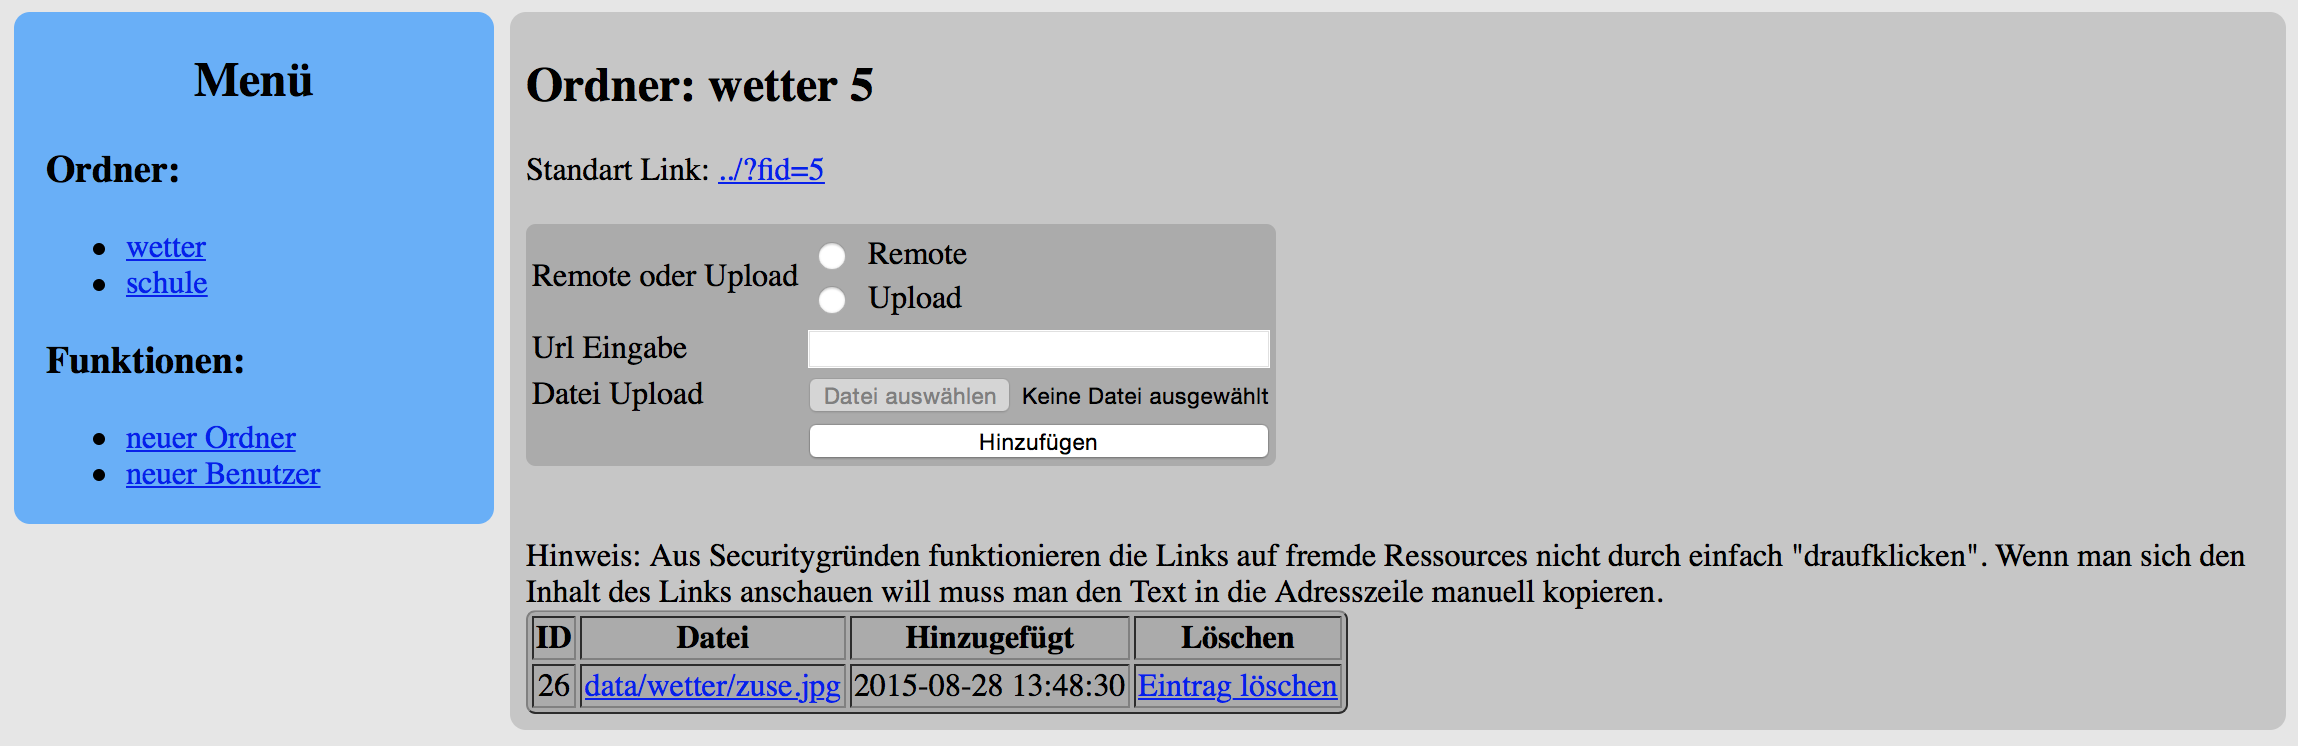
\includegraphics[width=\linewidth]{imgs/wms/wms_interface.png}
\end{center}
Diese Grafik zeigt das Erscheinungsbild des WMS-Interfaces. Es ist sichtbar
minimalistisch gehalten um robust zu sein, und auch die Wartung zu erleichtern.
Trotzdem ist es dynamisch, denn es erlaubt die Erstellung neuer Ordner und Nutzer,
und in allen Testszenarien konnte die Seite nicht zum Absturz gebracht werden.

\subsection{Generierte Grafiken}
\label{sub:Generierte Grafiken}
In diesem Abschnitt der Projektarbeit bestand wieder ein Bedarf nach automatisiert erzeugten Grafiken.
Einerseits ist das Wetter, ,,Weather'' ja schon namensgebend, somit ist der \vs -Teil meiner Arbeit schon relevant.
Zudem fand sich aber auch ein anderer Anlass Grafiken automatisiert zu generieren.
Das WMS System befindet sich im Foyer des Schulzentrum Kühlungsborns in dreifacher Ausführung.
Einer der Rechner soll als Geburtstagsanzeige genutzt werden.
Er zeigt also eine Reihe von Grafiken an, auf denen grafisch aufbereitete Tabellen aus Namen und Geburtsdaten der aktuellen Woche zu sehen sind.
Die Erzeugung dieser Grafiken erfolgte historisch im Hafen im Rahmen des Wahlpflichtfaches unter der Leitung von Dr. Ronald Eixmann.
Die Arbeit ist zeitaufwändig, und ein Schüler muss angelernt werden wie CoralDraw bedient wird.
Auch wenn die Fähigkeit dieses Programm benutzen zu können nicht unwichtig ist, ist die Arbeit die
Daten aus einer Tabelle zu lesen und in eine Maske einzutragen nicht notwendigerweise von einem Menschen abhängig.\\

\subsection{Application Programming Interface}
\label{sub:wmsapi}
Ein Application Programming Interface, kurz API, ist eine Schnittstelle zu einem größeren Programm
über eine Programmiersprache, welche nicht der des ursprünglichen Programmes entsprechen muss.
Über diese Schnittstelle soll dann die Ausführung von Aufgaben veranlasst werden.
Eine API ermöglicht also dann Entwicklern auf ihr Programm von außen zuzugreifen und es zu erweitern.
In dem Fall von WMS war eine API notwendig um von Programmen aus,
also nicht von \link{wms.viwetter.de}, Grafiken hochzuladen und zu verwalten.
Im Detail wird die API genutzt um die erzeugtet Geburtstagsgrafiken von einem Python Programm auf den Server zu laden und die Geburtstagsgrafikenschleife zu verwalten.
Die API auf Seiten des Servers ist in PHP geschrieben.
Auf diese API kann nun von außen jede Programmiersprache über GET und POST Requests des Hyper Text Transfer Protokolls zugreifen.
Eine dieser Programmiersprachenschnittstellen wurde für Python geschrieben.\\
Dieses System emuliert Großteils das REST-Ful Paradigmus.

\subsection{Erreichbarkeit} % WMS
Auch wenn der Server nicht globales Interesse erweckt soll er natürlich nicht nur im Hafen erreichbar sein.
Da Standorte sich auch verändern können,
und nicht dringend immer in Kühlungsborn liegen müssen, ist der Server über den Domainnamen \link{http://wms.viwetter.de} erreichbar. \\
Alle Funktionen die hier beschrieben wurden sind demnach auch von jedem internetfähigen PC erreichbar. Keiner der Computer hat Sonderrechte,
und es werden auch keine Cookies gespeichert.

\subsection{Sicherheit} % WMS
Da dieses System an öffentlichen Orten Anwendung finden soll,
muss gewährleistet sein, dass auf den Anzeigegeräten nur Daten angezeigt werden,
die von autorisierten Personen ausgewählt worden.
Außerdem soll der Service nicht ohne die Erlaubnis eines Administrators aufrufbar sein,
deshalb wurde ein Kontensystem implementiert.
Da die Client Computer automatisiert starten und gleich die richtigen Daten anzeigen sollen,
musste ein Protokoll entwickelt werden, welches sicher ist,
aber einem entferntem Rechner ermöglicht sich selbst anzumelden.
Um dafür zu sorgen, dass nur vollständig geladene Grafiken angezeigt werden muss
der Client beim Anzeigen selbst überprüfen ob die Grafik vorhanden ist.
Um sicherzustellen, dass die Anzeige auch im Rahmen der Projektarbeit aufgestellt
wurde muss sich der Rechner selbst authentifizieren.
Dafür muss auf ihm lokal ein Benutzername und ein
Authentifizierungshash gespeichert sein. Sein Passwort im Klartext ist dem Server nicht bekannt.
Selbst wenn der gesamte Datenbankinhalt veröffentlicht wird, kann weder ein Passwort
entschlüsselt werden\footnote{zumindest in einer Zeitspanne die
geringer als die Lebensdauer des Universums ist}, noch können Nutzer die das selbe Passwort haben
gruppiert werden.\\
Dieses Verhalten wurde erreicht indem das Passwort zusammen mit einem ,,Salt''-Wert gehash wird.
Dieser ,,Salt'' wird bei jedem Benutzer individuell
erzeugt und ist eine 256 Bit lange zufällige hexdezimale Zeichenkette.\\
Nicht nur der Server muss vor Angriffen geschützt werden, sondern auch der
Nutzer am anderen Ende der Leitung.
Teile des Interfaces nutzen JavaScript.
Diese Programmiersprache kann genutzt werden um Angriffe durchzuführen, und
auf jeder Seite die dynamische Inhalte anbietet gibt es die Gefahr das ein
Cross-Site-Scripting Angriff möglich ist.
Auf dem WMS-Interface wurden alle Vorbereitungen getroffen, dass dies nicht der
Fall ist. Jede Anfrage die dem Server geschickt wird, wird bevor sie in die Datenbank
geschrieben wird escaped. Escaping ist der Vorgang in dem Zeichen, die für den
Computer in einer Programmiersprache eine besondere Bedeutung haben so zu kennzeichnen,
dass sie nur als ,,Text'' gelesen und verstanden werden.
Um dann SQL-Injektionen zu verhindern werden alle Interaktionen mit der Datenbank
nicht über ,,normale'' SQL-Queries gehandhabt, sondern über Prepared-Statements
dürchgeführt.
\lstinputlisting[language=PHP]{example/prepared.php}
Ein Prepared Statement ist in SQL eine Befehlstruktur, in der Befehl und Inhalt
über zwei komplett getrennte Verbindungen transferiert werden.
Eine SQl-Injektion in der Form:
\lstinputlisting[language=PHP]{example/sqlinject.php}
kann nicht nur für Datenverlust, sondern auch für die Veröffentlichung
von Passwörtern und privaten Daten sorgen. Durch die Trennung von Befehl und Inhalt,
kann also mit geringfügig mehr Aufwand die Datensicherheit erheblich verbessert werden.
Aus diesem Grund werden serverseitig nur\footnote{Über Prepared Statements
können einige Daten nicht übertragen werden, an wenigen Stellen wird auf altmodische
Queries zurückgegriffen} Prepared Statements eingesetzt.

\subsection{Anzeige}
Die Anzeige erfolgt über den Browser, da ein Internetbrowser meist vorinstalliert ist
und die meisten Medien nativ anzeigen kann, ohne das ein zusätzliches Software packet
benötigt. \\
Nur einen Browser zu starten reicht allerdings nicht um das von mir verlangte Verhalten
zu erreichen. Der Browserstart soll direkt nach dem Bootvorgang erfolgen, der Rechner soll
dann auch so robust eingerichtet sein, dass sein Dateisystem bei dem wildesten Stromnetz
noch funktionsfähig bleibt.\\
Für diesen Zweck wurde eine abgewandelte Version des Open Source Raspbian Betriebssystems
entwickelt, das diesen Schritt automatisiert ausführt. Bei der Installation des
Rechners muss nur das Ziel eingegeben werden und die restliche Konfiguration
übernimmt das System. Um einem Rechner dieses Betriebssystem zu überspielen wird
wieder ein Raspberry Pi genutzt für den das Betriebssystem auf eine SD-Karte über
den Linux dd Befehl überspielt wird. Von dieser SD-Karte kann der Raspberry Pi
ohne Konfiguratin booten und die Einstellung des Ziels der Anzeige kann über eine
Tastatur an dem Pi selbst oder über eine SSH Verbindung erledigt werden.

\section{Makanya}

\subsection{Hintergrund} % Makanya
Der Hintergrund des Makanya.com Projektes ist eine Partnerschaft
zwischen der Kirchengemeinde Kühlungsborn und Tansania,
sowie der Partnerschaft zwischen der Kirchengemeinde und dem Schulzentrum Kühlungsborns.
Der Pastor Kühlungsborns, Matthias Borchert,
suchte den Kontakt zum \jf Team über das Schulzentrum.
Nach einer kurzen Bekanntmachung durch Frau Schmidt war die Zusammenarbeit besiegelt.\\
Eine Domain (\link{makanya.com}) von strato.de war bereits vorhanden% TODO Quelle + Preise
% Server: strato.de
und ein WordPress Blog \link{kulungsi.com}.
Die Website musste technisch aufbereitet werden, und eine englische Übersetzung war notwending.
Diese Website sollte dann als Anlaufpunkt für alle Projektteilnehmer, Interessenten und Schüler sein.
% Sprache: Deutsch, Englisch, Zusammenarbeit (Dolmetschering: Frau Wieck)
Aus dieser Spezifizierung ergeben sich die Anforderungen an die Programmierung:\\
Der Inhalt der Website muss auf Deutsch und Englisch sein, beide Versionen weitestgehend identisch.
Weiterhin soll die Webseite einfach bedienbar sein,
damit auch technisch unbegabte Schüler und Verwaltungsmitglieder sich durch die Webseite navigieren können sollen.
Damit die Seite auch in Tansania erreichbar ist müssen die Datenformate optimiert werden.\\
% Programmierung: PHP, HTML, MySQL
% Mehr Programmierung...?
% Beiprogramm: Schulzentrum -> Spendenlauf, Besuch der Tansanianer, Meetings, Auswertung
Somit stellt diese Arbeit ein Teil eines größeren Projektes dar.
Dieses Projekt beinhaltet die Partnerschaft von der Kirchengemeinde mit dem Schulzentrum und Makanya in Tansania.
Andere Aspekte beinhalten den Schüleraustausch und Besuch der Tansanianer,
sowie ein von der Schule organisierter Spendenlauf der die Finanzierung des Fluges ermöglichte.

\subsection{Methodik} % Makanya
% Aufteilung:
% Markus: Programmierung, Öffentlichkeitsarbeit, Infos

% Umgebung: Sublime Text, PHPmyAdmin,
% Hilfe: php.net (erstes PHP Projekt)
% Sicherheit: sha256 Schlüssel, TODO Vortrag herauskramen!
Die hauptsächliche Arbeit wurde in der Programmiersprache PHP erledigt.
Da das Ergebnis als Website erreichbar sein sollte,
war von Anfang an klar, dass die Seite am Ende den Nutzer in HTML, CSS und JavaScript
erreichen müsse.
Die Programmierung des Backends geschah in Kürze nach dem ersten Treffen und der Übergabe der Logindaten.
Die Website war funktionsfähig sobalt sie die Informationen auf Kulungsi.com wiederspiegelte.
Da dieses Zeil schnell erreicht war, sollte nun weiterführend eine Art soziales Netzwerk zwecks Austausch im Hintergrund errichtet werden.
Dieser Teil der Website ist zum Zeitpunkt der Setzung noch nicht fertiggestellt, die grundlegenden
Funktionen: Chats, Accounts, Gruppen und weitere Kleinigkeiten sind allerdings schon funktionstüchtig.\\
Die Entwicklung wurde durch den Texteditor Sublime Text erleichtert. Als Testserver diente ein von mir sonst privat genutzter Raspberry Pi,
wobei ich allerdings von vornherein auf der von Strato.de zur Verfügung gestellten Datenbank arbeitete.
Außerdem hervorstechend ist das erste größere Treffen des Tansaniakreises Kühlungsborns, dem ich beiwohnte.
Meine Aufgabe war es dem Kern der Gemeinde meine Fortschritte zu präsentieren.
Eine Präsentation mit für diesen Anlass erzeugten Grafiken diente um die Entwicklung einer Website
sowie die damit verbundenen Schwierigkeiten, Limitationen und Abläufe visuell zu erläutern.


\subsection{Ergebnis} % Makanya
Das Ergebnis dieses Projektes ins die Webseite, die statische Informationen über Makanja bereitstellt.
Dazu gibt es im Hintergrund eine minimale Version eines sozialen Netzwerkes mit einem offenen und geschlossenen Chat.
Außerdem wurden alle von dem Projekt erwarteten Sicherheitsbedingungen eingehalten.
Auf der Sicherheit liegt bis heute noch der Fokus:
solange die Website erreichbar ist und die richtigen Informationen anzeigt ist ihre Aufgabe erfüllt.
Die Autoritätspersonen und Lehrer bekamen außerdem die Möglichkeit die ihnen untergestellten Schüler zu verwalten.
Somit konnte auch die Idee des Konten- und Rechtesystems umgesetzt werden.\\
Da dieses Teilgebiet der Arbeit nicht viel Beaufsichtigung und stetige Entwicklung verlangt ist
es im Verlauf der Arbeit auf der Prioritätenliste langsam abgestiegen.
\begin{center}
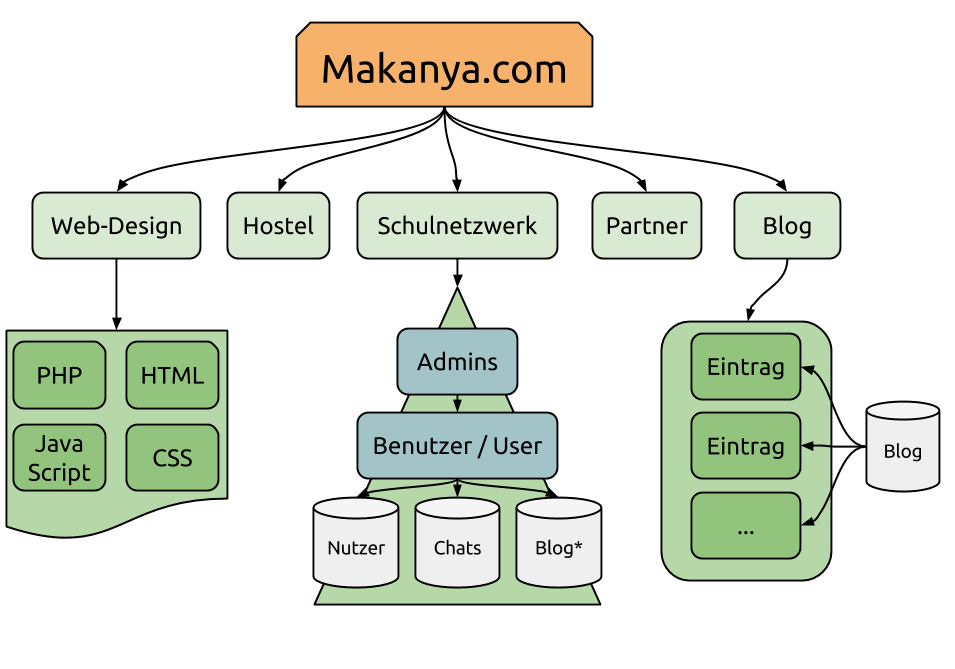
\includegraphics[width=\linewidth]{imgs/makanyaOverview.png}
\end{center}


\newpage
\printbibliography

% NOTE Großteil des Quellcodes muss in den Anhang
\newpage
\section{Anhang}
Der komplette aktualisierte Quelltext ist für AuVi / \vs\, unter \link{github.com/tibyte/auvi-hub} und für das Weather-Monitoring-System unter \link{github.com/tibyte/apewms} hochgeladen und frei verfügbar. Der grafische Teil des Weather-Monitoring-Systems und die Python API ist unter \link{github.com/tibyte/autowkid} veröffentlicht.\\
Stellen, auf die im Laufe dieser Arbeit häufiger verwiesen werden und sie deshalb größere Wichtigkeit genießen sind im Folgenden Anhang zu finden. Zudem befinden sich nach den Quelltexten eine Reihe von Grafiken, welche von \vs\, beziehungsweise WMS erzeugt wurden.


% Hallo!

\end{document}
